% Based on the template of https://github.com/fizixmastr 

\documentclass[A4,11pt]{article}
%\documentclass[letterpaper,11pt]{article} %For use in US
\usepackage{latexsym}
\usepackage[empty]{fullpage}
%\usepackage{titlesec}
\usepackage{marvosym}
\usepackage[usenames,dvipsnames]{color}
\usepackage{verbatim}
\usepackage{enumitem}
\usepackage[hidelinks]{hyperref}
\usepackage[english]{babel}
\usepackage{tabularx}
\usepackage{tikz}
\usepackage{titlesec}
%\input{glyphtounicode}

\begin{comment}
  comments
\end{comment}


%-----FONT OPTIONS-------------------------------------------------------------
\begin{comment}
The font of the document will impact not just how readable it is, but how it is
perceived. In the "The Craft of Scientific Writing" by Michael Alley, shares a
common fonts for publication as well as their use. I have chosen to use
Palatino for its legibility, some others are given below. There is far too much
about typography to discus here. Note: serif fonts have short projecting
strokes, sans-serif fonts are sans (without) these strokes.
\end{comment}


% serif
 %\usepackage{palatino}
  %\usepackage{times} %This is the default as well
%\usepackage{charter}
\usepackage{newtxtext,newtxmath}

% sans-serif
% \usepackage{helvet}
% \usepackage[sfdefault]{noto-sans}
% \usepackage[default]{sourcesanspro}

%-----PAGE SETUP---------------------------------------------------------------

% Adjust margins
\addtolength{\oddsidemargin}{-1cm}
\addtolength{\evensidemargin}{-1cm}
\addtolength{\textwidth}{2cm}
\addtolength{\topmargin}{-1cm}
\addtolength{\textheight}{2cm}

% Margins for US Letter size
%\addtolength{\oddsidemargin}{-0.5in}
%\addtolength{\evensidemargin}{-0.5in}
%\addtolength{\textwidth}{1in}
%\addtolength{\topmargin}{-.5in}
%\addtolength{\textheight}{1.0in}

\urlstyle{same}

\raggedbottom
\raggedright
\setlength{\tabcolsep}{0cm}

% Sections formatting
\titleformat{\section}{
  \vspace{-4pt}\scshape\raggedright\large
}{}{0em}{}[\color{black}\titlerule \vspace{-5pt}]

% Ensure that .pdf is machine readable/ATS parsable
%\pdfgentounicode=1

%-----CUSTOM COMMANDS FOR FORMATTING SECTIONS----------------------------------
\newcommand{\CVItem}[1]{
  \item\small{
    {#1 \vspace{-2pt}}
  }
}

\newcommand{\CVSubheading}[4]{
  \vspace{-2pt}\item
    \begin{tabular*}{0.97\textwidth}[t]{l@{\extracolsep{\fill}}r}
      \textbf{#1} & #2 \\
      \small#3 & \small #4 \\
    \end{tabular*}\vspace{-7pt}
}

\newcommand{\CVSubSubheading}[2]{
    \item
    \begin{tabular*}{0.97\textwidth}{l@{\extracolsep{\fill}}r}
      \text{\small#1} & \text{\small #2} \\
    \end{tabular*}\vspace{-7pt}
}

\newcommand{\CVSubItem}[1]{\CVItem{#1}\vspace{-4pt}}

\renewcommand\labelitemii{$\vcenter{\hbox{\tiny$\bullet$}}$}

\newcommand{\CVSubHeadingListStart}{\begin{itemize}[leftmargin=0.5cm, label={}]}
% \newcommand{\resumeSubHeadingListStart}{\begin{itemize}[leftmargin=0.15in, label={}]} % Uncomment for US
\newcommand{\CVSubHeadingListEnd}{\end{itemize}}
\newcommand{\CVItemListStart}{\begin{itemize}}
\newcommand{\CVItemListEnd}{\end{itemize}\vspace{-5pt}}

\newenvironment{paperlist}
{ \begin{itemize}[leftmargin=0.8cm, label={$\bullet$}]
    \setlength{\itemsep}{1pt}
    \setlength{\parskip}{1pt}
    \setlength{\parsep}{1pt}     }
{ \end{itemize}                  } 


%------------------------------------------------------------------------------
% CV STARTS HERE  %
%------------------------------------------------------------------------------
\begin{document}

%-----HEADING------------------------------------------------------------------
\begin{comment}
In Europe it is common to include a picture of ones self in the CV. Select
which heading appropriate for the document you are creating.
\end{comment}

\begin{minipage}[c]{0.05\textwidth}
\-\
\end{minipage}
\begin{minipage}[c]{0.2\textwidth}
\begin{tikzpicture}
    \clip (0,0) circle (1.75cm);
    \node at (0.2,-.5) {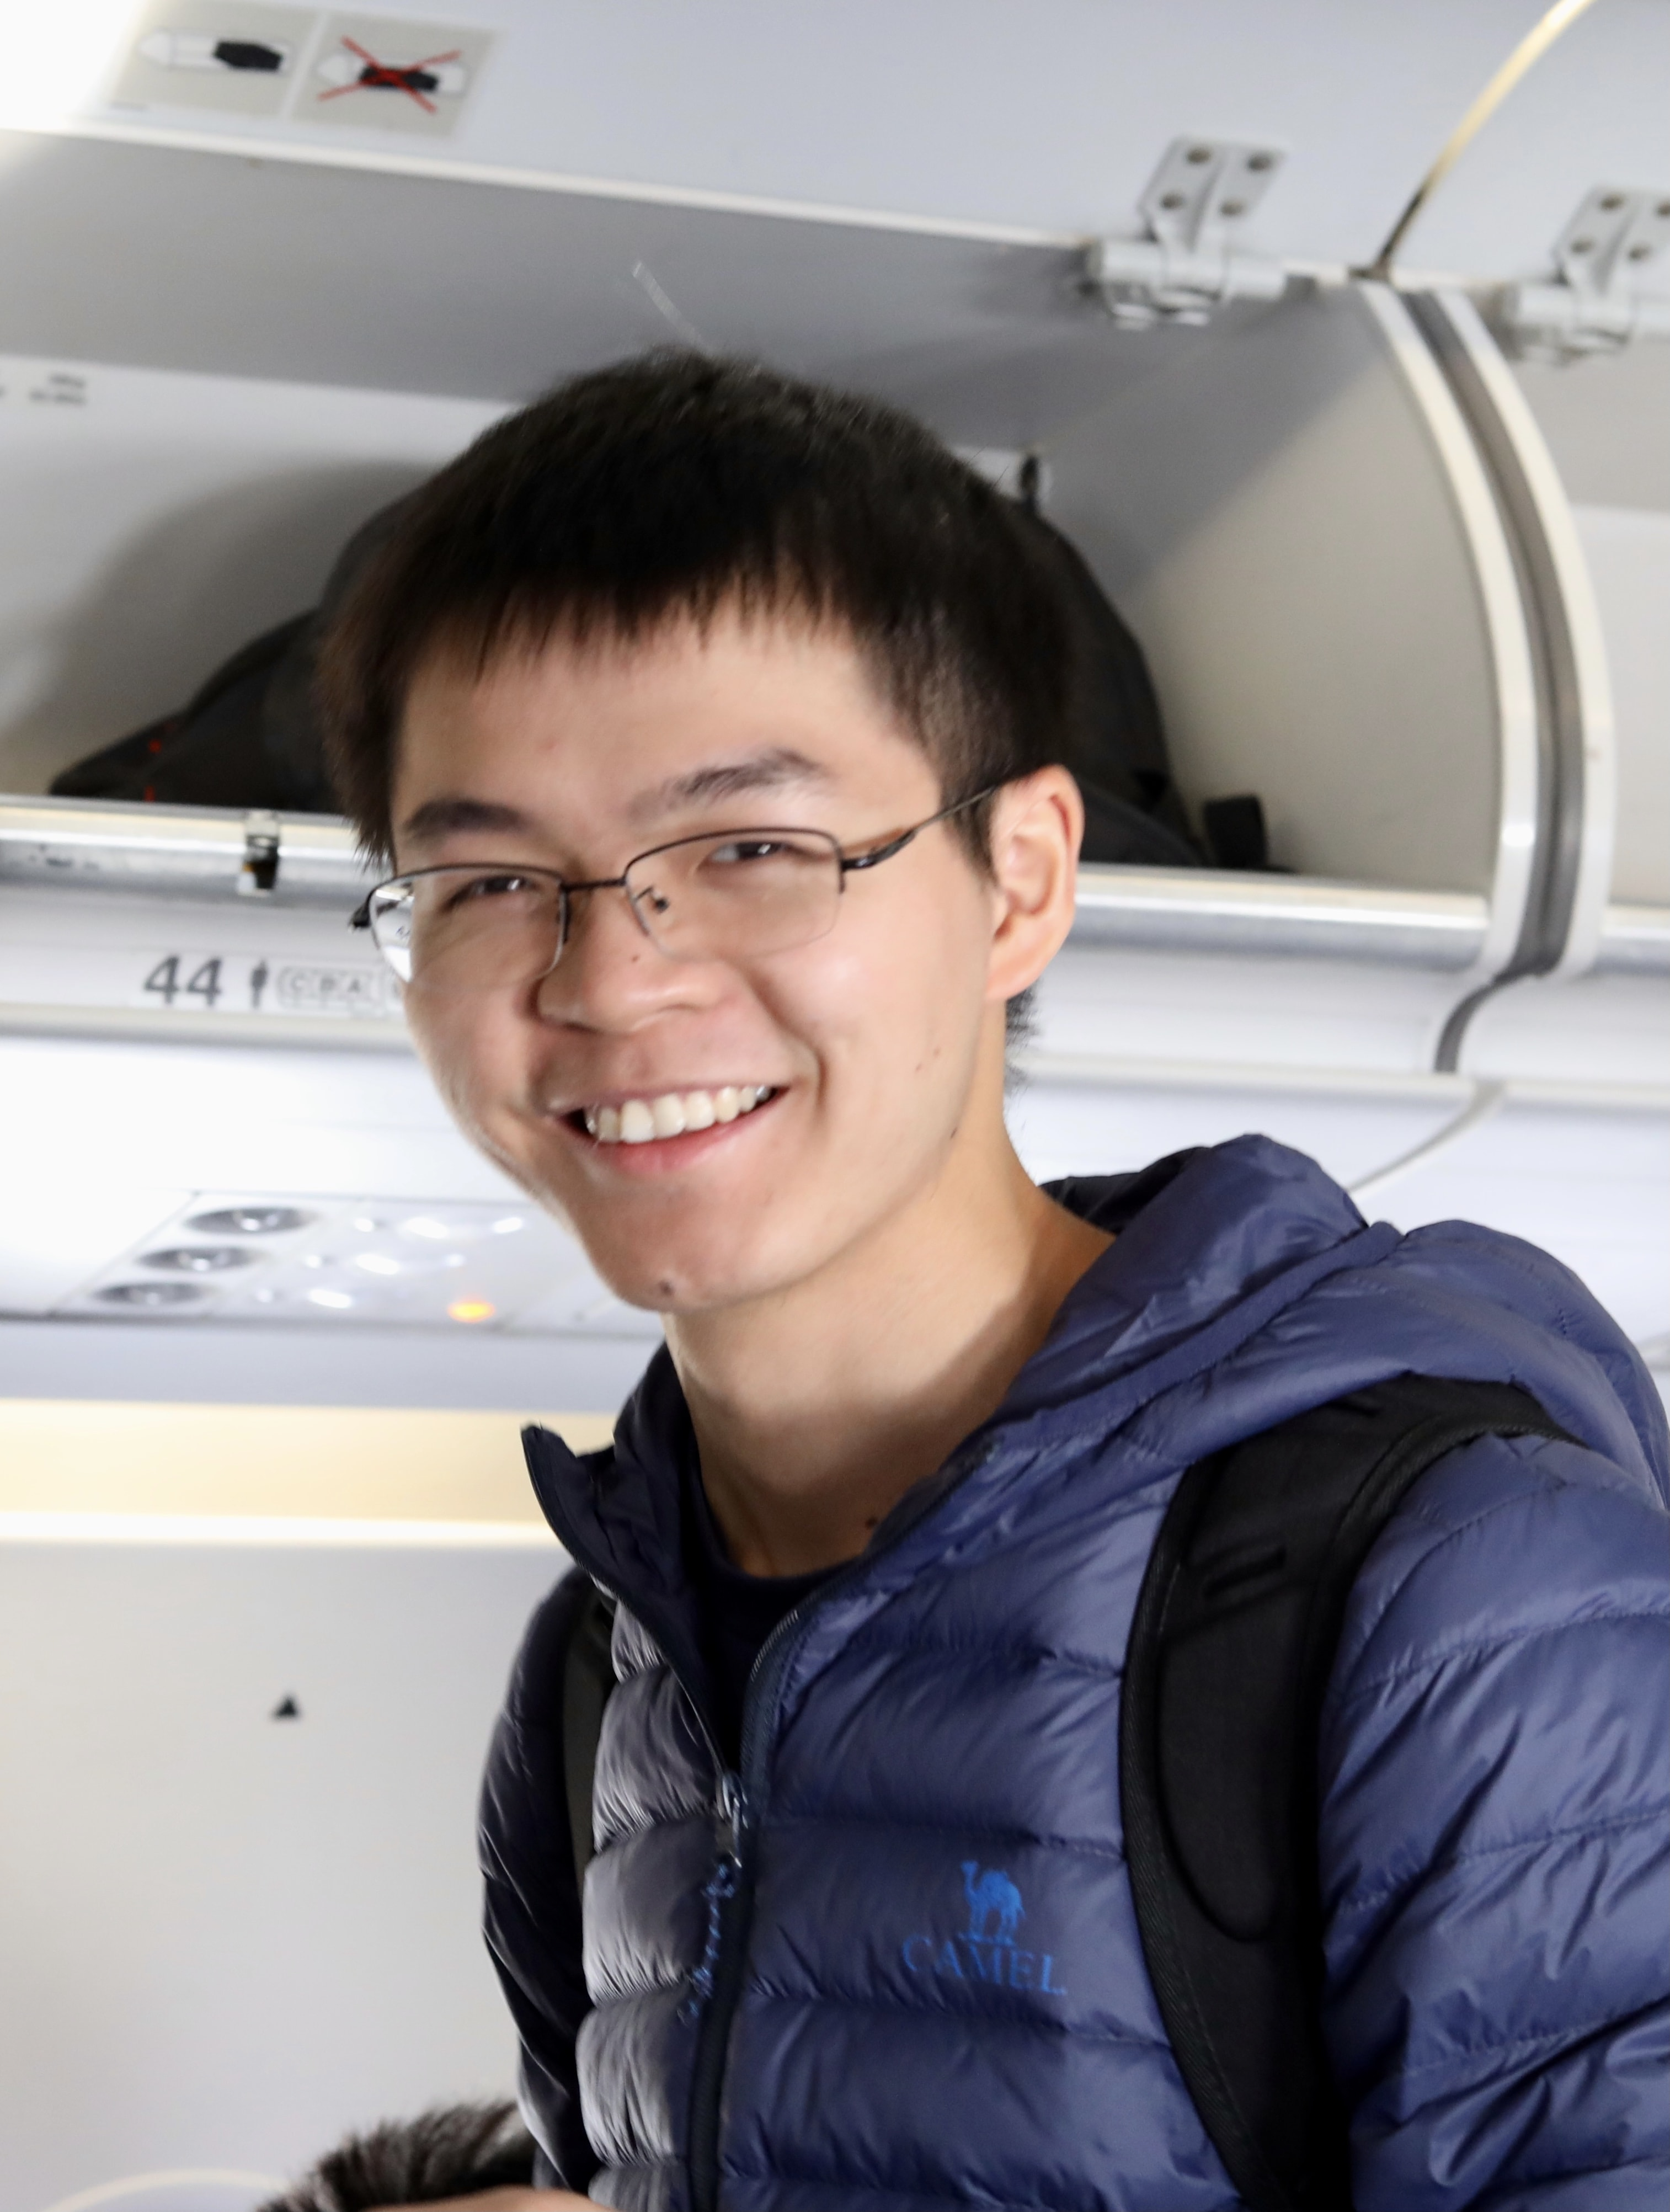
\includegraphics[width = 5cm]{Jianhang.jpg}}; 
    % if necessary the picture may be moved by changing the at (coordinates)
    % width defines the 'zoom' of the picture
\end{tikzpicture}
\hfill\vline\hfill
\end{minipage}
\begin{minipage}[c]{0.6\textwidth}
    \textbf{\Huge Jianhang CHEN} \\ \vspace{1pt} 
    % \scshape sets small capital letters, remove if desired
    \small{+49 1627363870} \\
    \href{mailto:Jianhang.Chen@eso.org}{\underline{Jianhang.Chen@eso.org}}\\
    % Be sure to use a professional *personal* email address
    %\href{https://www.linkedin.com/in/charles-rambo/}{\underline{linkedin.com/in/charles-rambo}} \\
    \href{https://cjhastro.github.io}{\underline{https://cjhastro.github.com}}\\
    % you should adjust you linked in profile name to be professional and recognizable
    \href{https://github.com/cjhang}{\underline{github.com/cjhastro}} \\
    Karl-Schwarzschild-Strasse 2\\ 85748, Garching bei München, Germany
\end{minipage}

% Without picture
%\begin{center}
%    \textbf{\Huge \scshape Charles Rambo} \\ \vspace{1pt} %\scshape sets small capital letters, remove if desired
%    \small +1 123-456-7890 $|$ 
%    \href{mailto:you@provider.com}{\underline{you@provider.com}} $|$\\
%    % Be sure to use a professional *personal* email address
%    \href{https://linkedin.com/in/your-name-here}{\underline{linkedin.com/in/charles-rambo}} $|$
%    % you should adjust you linked in profile name to be professional and recognizable
%    \href{https://github.com/fizixmastr}{\underline{github.com/fizixmastr}}
%\end{center}



\begin{comment}
This CV was written for specifically for positions I was applying for in
academia, and then modified to be a template.

A standard CV is about two pages long where as a resume in the US is one page.
sections can be added and removed here with this in mind. In my experience, 
education, and applicable work experience and skills are the most import things
to include on a resume. For a CV the Europass CV suggests the categories: Work
Experience, Education and Training, Language Skills, Digital Skills,
Communication and Interpersonal Skills, Conferences and Seminars, Creative Works
Driver's License, Hobbies and Interests, Honors and Awards, Management and
Leadership Skills, Networks and Memberships, Organizational Skills, Projects,
Publications, Recommendations, Social and Political Activities, Volunteering.

Your goal is to convey a who, what , when, where, why for every item you share. 
The who is obviously you, but I believe the rest should be done in that order.
For example below. An employer cares most about the degree held and typically 
less about the institution or where it is located (This is still good 
information though). Whatever order you choose be consistent throughout.
\end{comment}

%-----EDUCATION----------------------------------------------------------------
\section{Education}
  \CVSubHeadingListStart
%    \CVSubheading % Example
%      {Degree Achieved}{Years of Study}
%      {Institution of Study}{Where it is located}
    \CVSubheading
      {{PhD of Science $|$ \emph{\small{Astrononmy}}}}{Sep. 2020 -- Aug. 2023}
      {European Southern Observatory $|$ Supervisor: Prof. Rob Ivison}{Garching, Germany}
    \CVSubheading
      {{Master of Science $|$ \emph{\small{Astronomy}}}}{Sep. 2017 -- Jun. 2020}
      {Nanjing University $|$ Supervisor: Prof. Yong Shi \& Prof. Zhi-yu Zhang}{Nanjing, China}
    \CVSubheading
      {{Bachelor of Science $|$ \emph{\small{Physics}}}}{Sep. 2013 -- May. 2017}
      {Lanzhou University}{Lanzhou, China}
  \CVSubHeadingListEnd

%-----WORK EXPERIENCE----------------------------------------------------------
\begin{comment}
try to briefly explain what you did and why it is relevant to the position you
are seeking
\end{comment}

\section{Telescope Proposals and Observing Experience}
{\bf PI Proposals}:\\
\vspace{-0.8em}
\begin{paperlist}
    \item {\bf IRAM30m} Summer 2022 Delta, 095-22:  The tip of the iceberg? 34.4\,hrs, {\bf (PI. Jianhang Chen, A priority)}.
    \item {\bf ALMA} Cycle-9, 2022.1.00495.S: \emph{Isotopic constraints on the IMF in the most extreme star-forming environments in the Universe}, 23.7\,hrs, {\bf (PI: Jianhang Chen, A priority)}. 
    \item {\bf JCMT} 22A, M22AP002: Revealing the structure around a putative new SMG proto-cluster core, 8.5\,hrs, {\bf (PI: Jianhang Chen, B priority)}.
    \item {\bf ALMA} Cycle-8, 2021.1.00458.S: \emph{Dust polarisation in distant, star-foming galaxies: a transformative survey of the viable targets}, 25.1\,hrs, {\bf (PI: Jianhang Chen, B priority)}. 
    \item {\bf NEOMA} Summer 2020, S20BB: \emph{Searching for molecular gas in HI-rich red spirals}, 2.8\,hrs, {\bf (PI: Jianhang Chen, B priority)}. 
\end{paperlist}

{\bf Co-I Proposals}:\\
\vspace{-0.8em}
\begin{paperlist}
    \item {\bf ALMA} Cycle-8, 2021.1.00018.S: \emph{Exploiting a snapshot survey of the 3,083 reddest Herschel sources to reveal distant protoclusters}, 30.6\,hrs, (PI. R. Ivison, CoI: Jianhang Chen).
    \item {\bf ALMA} Cycle-8, 2021.1.01342.S: \emph{[CI] as a molecular gas tracer in star forming galaxies at high redshift}, 9.6\,hrs, (PI: M. Castillo, CoI: Jianhang Chen)
    \item {\bf VLA} 2020B, 20B-180: \emph{Off-nuclear star formation in a gas-rich low-mass S0 galaxy}, 27\,hrs, (PI: Zhengyi Chen, CoI: Jianhang Chen)
    \item {\bf NOEMA} Summer 2020, S20CK: \emph{Exploiting a snapshot survey of the 3,083 reddest Herschel sources to reveal distant protoclusters}, 26\,hrs, (PI: Vinodiran Arumgam, CoI: Jianhang Chen)
    \item {\bf IRAM30m} Summer 2020, 062-20: \emph{Do Changing-look AGNs reside in the gas-rich environment?}, 23.5\,hrs, (PI: Xiaoling Yu, CoI: Jianhang Chen)
\end{paperlist}

{\bf Observing Experience}:\\
\vspace{-0.8em}
\begin{paperlist}
    \item IRAM30m, NIKA2, 6 nights, 18-25 Oct. 2022
\end{paperlist}


%-----PROJECTS AND RESEARCH----------------------------------------------------
\begin{comment}
Ideally the title of the work should speak for what it is. However if you feel
like you should explain more about why the project is applicable to this job,
use item list as is shown in the work experience section.
\end{comment}

%-----RESEARCH EXPERIENCE------------------------------------------------------
\section{Research Experience}
  \CVSubHeadingListStart
    \CVSubheading
      {11th NOEMA Interferometry School}{21-25 Nov.~2021}
      {Winter School}{Grenoble, France}
    \CVSubheading 
      {Short term visit, Durham University/Physics department}{14-24 Sep. 2022}
      {Host: Prof. Mark Swinbank Topic: dynamical modeling}{Durham, UK}
    \CVSubheading 
      {Astrophysics, Formation and Evolution of Galaxy cluster Across Cosmic Time}{23 Nov.-1 Dec.~2021}
      {Winter School}{Tenerife, Spain}
    \CVSubheading 
      {10th IRAM 30-meter School on Millimeter Astronomy}{15-23 Nov.~2021}
      {Winter School}{Online}
    \CVSubheading
      {Astrostatistics and R training}{09-13 Jul.~2018}
      {The 2nd East Asian Astrostatistics International Conference (EAAIC2018)}{Nanjing, China}
  \CVSubHeadingListEnd


\section{Conference and Seminar Talks}
  \CVSubHeadingListStart
%    \CVSubheading
%      {Title of Work}{When it was done}
%      {Institution you worked with}{unused}
    \CVSubheading
      {ALMACAL IX: multi-band ALMA survey for dusty star-forming galaxies}{15--23~Dec. 2022}
      {A half-century of millimeter and submillimeter astronomy}{Miyakojima, Japan}
    \CVSubheading
      {ALMACAL: Number counts and the resolved fractions of the CIB}{3--4~Mar. 2022}
      {Meeting of ALMA Young Astronomers}{Online}
    \CVSubheading
      {Submillimetre number counts}{5--6~Nov. 2021}
      {12th IMPRS Symposium}{Garching, Germany}
    \CVSubheading
      {The spatial extension of AGN narrow line regions}{1--4 Apr. 2019}
      {MaNGA Collaboration Meeting}{Oxford, UK}
  \CVSubHeadingListEnd

%-----CONFERENCES AND PRESENTATIONS--------------------------------------------
\begin{comment}
Again the title should have already been enough, but if it is necessary to add
descriptions maintain the consistency from prior sections
\end{comment}

\section{Posters}
  \CVSubHeadingListStart
%    \CVSubheading % Example
%      {Work Presented}{When}
%      {Occasion}{}
    \CVSubheading
      {ALMACAL: A `free' submillimetre galaxy survey}{3--5~May. 2022}
      {PoSTER 2022 - Galaxy Evolution (Best poster award)}{Online}
    \CVSubheading
      {ALMACAL: Hunting for regions over-dense in SMGs}{23~Nov.--1~Dec. 2021}
      {XXXII Canary Islands Winter School of Astrophysics}{Tenerife, Spain}
  \CVSubHeadingListEnd



%-----TEACHING EXPERIENCE------------------------------------------------------
\begin{comment}
Section is here as it applied to my application for positions in academia. 
Remember to tailor the resume for to the position.
\end{comment}

%-----COMMUNITY INVOLVEMENT----------------------------------------------------
\section{Community Involvement}
  \CVSubHeadingListStart
%    \CVSubheading %Example
%      {What you did}{When you worked there}
%      {Who you worked for}{Where they are located}
    \CVSubheading
      {Scientific Assistant at ESO OPC P110}{May. 2022}
      {Helping to organise pannel discussion}{}
    \CVSubheading
      {Scientific Assistant at ESO OPC P109}{Nov. 2021}
      {Helping to organise pannel discussion}{}
    \CVSubheading
      {Organisor of student session of Munich Joint Astronomy Colloquium}{Nov. 2021}
      {Helping to coodinate the discussion between students and the speaker}{}
    \CVSubheading
      {Member of LOC for the 11th IMPRS Symposium}{May 2021}
      {Helping to organise meeting schedule}{}

    \CVSubheading
      {Scientific referee for Publications of the Astronomical Society of Japan}{2020}
      {}{}
  \CVSubHeadingListEnd

%-----HONORS AND AWARDS--------------------------------------------------------
\section{Awards and Scholarship}
  \CVSubHeadingListStart
%    \CVSubheading %Example
%      {What}{When}
%      {Short Description}{}
    \CVSubheading
      {International Max-Planck Research Scholarship (IMPRS) on Astrophysics}{2020-2023}
      {Grant for PhD study}{}
    \CVSubheading
      {Excellence Scholarship}{Spring 2019}
      {Nanjing University}{}
    \CVSubheading
      {Outstanding Graduates Award}{Spring 2017}
      {Lanzhou University}{}
    \CVSubheading
      {National Encouragement Scholarship}{2015,2016}
      {Merit based scholarship for colleage students in China}{}
    \CVSubheading
      {The First Prize Scholarships}{Spring 2014}
      {Lanzhou University}{}
  \CVSubHeadingListEnd


%-----SKILLS-------------------------------------------------------------------
\begin{comment}
This section is compressed from the various skills sections that Euro CV
recommends.
\end{comment}

\section{Skills}
 \begin{itemize}[leftmargin=0.5cm, label={}]
    \small{\item{
     \textbf{Languages}{: Chinese (Native), English (C1)} \\
     \textbf{Programming}{: Python (NumPy, SciPy, Matplotlib, Pandas), MATLAB, Mathematica} \\
     \textbf{Document Creation}{: HTML, LaTex, Markdown} \\
     \textbf{Software}{: pPXF, CASA, CARTA, DS9, BBarolo, Galpak}
    }}
 \end{itemize}


\section{Publications}
{\bf First author papers:}\\
\vspace{-0.8em}
\begin{paperlist}
    \item ``ALMACAL X: Extreme over-densities are not always signposts to proto-clusters -- a cautionary tale" Chen, Ivison, Zwaan et al. MNRAS. (in submission)
    \item ``ALMACAL IX: multi-band ALMA survey for dusty star-forming galaxies and the resolved fractions of the cosmic infrared background" Chen, Ivison, Zwaan et al. MNRAS, (2022), arXiv:2210.09329 
    \item ``The spatial extension of extended narrow line regions in MaNGA AGN" Chen, Shi, Dempsey et al. MNRAS, 489, 855 (2019)
\end{paperlist}


{\bf Co-author papers:}\\
\vspace{-0.8em}
\begin{paperlist}
    \item ``The H I gas disc thickness of the ultra-diffuse galaxy AGC 242019” Li, Shi, Zhang et al. MNRAS, 516, 4220 (2022)
    \item ``ALMACAL: Surveying the Universe with ALMA Calibrator Observations" Zwaan, Ivison, Peroux et al. The Messenger, 186, 10 (2022)
    \item ``The major mechanism to drive turbulence in star-forming galaxies” Yu, Bian, Krumholz et al. MNRAS, 505, 5075 (2021)
    \item ``Probing possible effects of circumgalactic media on the metal content of galaxies through the mass-metallicity relationship” Zhai, Shi, Chen et al. MNRAS, 504, 1959 (2021)
    \item ``A Cuspy Dark Matter Halo” Shi, Zhang, Wang et al. ApJ, 909, 20 (2021)
    \item ``The impact of merging on the origin of kinematically misaligned and counter-rotating galaxies in MaNGA” Li, Shi, Bizyaev et al. MNRAS, 501, 14 (2021)
    \item ``Host galaxy properties of changing-look AGNs revealed in the MaNGA survey” Yu, Shi, Chen et al. MNRAS, 498, 3985 (2020)
    \item ``What drives the velocity dispersion of ionized gas in star-forming galaxies?” Yu, Shi, Chen et al. MNRAS, 486, 4463 (2019)
    \item ``An early-type galaxy with an inner star-forming disc” Li, Shi, Chen et al. MNRAS, 480, 1705 (2018)
\end{paperlist}
%------------------------------------------------------------------------------
\end{document}
